\documentclass[border=10pt]{standalone}
\usepackage{tikz}
\usetikzlibrary{arrows.meta, shapes, calc}

\begin{document}

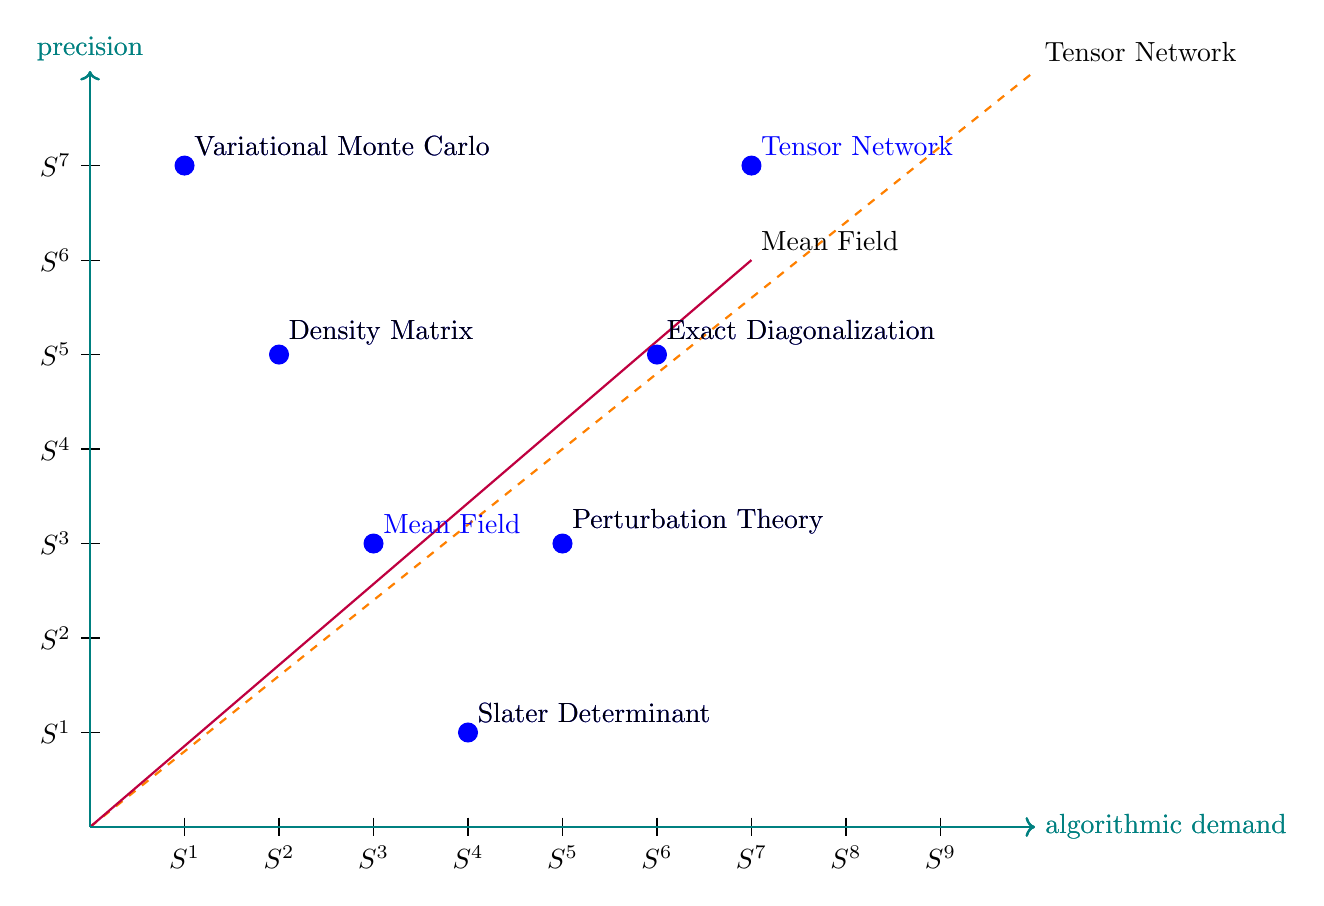
\begin{tikzpicture}[scale=1.2]
    % Axes
    \draw[->, thick, teal] (0,0) -- (10,0) node[right] {algorithmic demand};
    \draw[->, thick, teal] (0,0) -- (0,8) node[above] {precision};
    
    % Grid
    \foreach \x in {1,...,9} \draw (\x,0.1) -- (\x,-0.1) node[below] {$S^\x$};
    \foreach \y in {1,...,7} \draw (0.1,\y) -- (-0.1,\y) node[left] {$S^\y$};
    
    % Lines
    \draw[dashed, thick, orange] (0,0) -- (10,8);
    \draw[thick, purple] (0,0) -- (7,6);
    
    % Points and labels
    \foreach \x/\y/\label in {1/7/Variational Monte Carlo, 2/5/Density Matrix, 3/3/Mean Field, 4/1/Slater Determinant, 5/3/Perturbation Theory, 6/5/Exact Diagonalization, 7/7/Tensor Network}
        \filldraw[blue] (\x,\y) circle (0.1) node[above right] {\label};
    
    % Arrows
    \draw[->, thick, teal] (0,0) -- (0,8) node[above] {precision};
    \draw[->, thick, teal] (0,0) -- (10,0) node[right] {algorithmic demand};
    
    % Annotations
    \node[above right] at (10,8) {Tensor Network};
    \node[above right] at (7,6) {Mean Field};
    \node[above right] at (4,1) {Slater Determinant};
    \node[above right] at (5,3) {Perturbation Theory};
    \node[above right] at (6,5) {Exact Diagonalization};
    \node[above right] at (2,5) {Density Matrix};
    \node[above right] at (1,7) {Variational Monte Carlo};
    
\end{tikzpicture}

\end{document}